\section{引言}
\label{sec:intro}

\IEEEPARstart{过}{去}五年，深度学习系统从「把模型跑起来」变成了「把一个万卡集群、一个千亿参数模型和一组严格的
服务等级目标（SLO）同时摆平」。GPT-3 一类模型的训练算力达到 $10^{23}$ FLOP 量级~\cite{brown2020gpt3}，Llama~3 的最大模型
在约 1.6 万张 H100 上训练了 15.6T token~\cite{dubey2024llama3}；推理侧，KV cache 的显存管理与调度已经成为
独立的系统研究方向~\cite{kwon2023vllm,yu2022orca,agrawal2024sarathi,zhong2024distserve}。相应地，ML 系统岗位的面试形成了一种
相当稳定的风格：面试官很少问「某篇论文第几节写了什么」，而是问「这个数字从哪来、瓶颈在哪、换一种做法会怎样」。

这种风格背后有清楚的工程理由。大模型系统的设计空间巨大，但绝大多数候选方案可以在白板上用几行算术排除：
一个 7B 模型用混合精度 Adam 训练至少需要 $16N=112$~GB 的静态显存，单张 80~GB GPU 放不下；
一个 batch 为 1 的 decode 步要把 16~GB 权重从 HBM 读一遍，在 3.35~TB/s 的 H100 上下界约 5~ms；
8 卡之间 ring all-reduce 14~GB 梯度，即使走 450~GB/s 的 NVLink 也要约 54~ms。能做这类估算的工程师，
才能在没有 profiler 之前就知道该优化哪里，也才能判断一篇论文的加速比是否可信。

\subsection{三个问题的框架}

本文把 ML 系统的几乎全部问题归约为三个问题（图~\ref{fig:map}）：
\begin{enumerate}
\item \textbf{算得过来吗}（compute）：FLOPs、算术强度、roofline。若不会这一层，所有关于「为什么 decode 受访存限制」
的回答都只能背诵。
\item \textbf{放得下吗}（memory）：权重、梯度、优化器状态、激活与 KV cache 各占多少字节，怎么切分、重算或卸载。
\item \textbf{传得过来吗}（communication）：all-reduce 的通信量、流水线气泡、PCIe/NVLink/InfiniBand 带宽与拓扑。
\end{enumerate}
形式化地，一个训练步或推理步的时间下界和显存约束可以写成
\begin{equation}
\begin{gathered}
T_{\text{step}} \gtrsim \max\!\left(\frac{F}{P_{\text{peak}}},\ \frac{B_{\text{HBM}}}{\mathrm{BW}_{\text{HBM}}},\
\frac{B_{\text{net}}}{\mathrm{BW}_{\text{net}}}\right),\\
M_{\text{static}} + M_{\text{dyn}} \le M_{\text{HBM}},
\end{gathered}
\label{eq:three}
\end{equation}
其中 $F$ 为浮点运算量，$B_{\text{HBM}}$、$B_{\text{net}}$ 分别为 HBM 与网络上搬运的字节数。式~\eqref{eq:three}
假设计算、访存与通信可以完全重叠；不能重叠时取和而不是取最大值。本文后续章节几乎都是在给这个式子的
某一项代入具体的系统设计。

\begin{figure*}[!t]
\centering
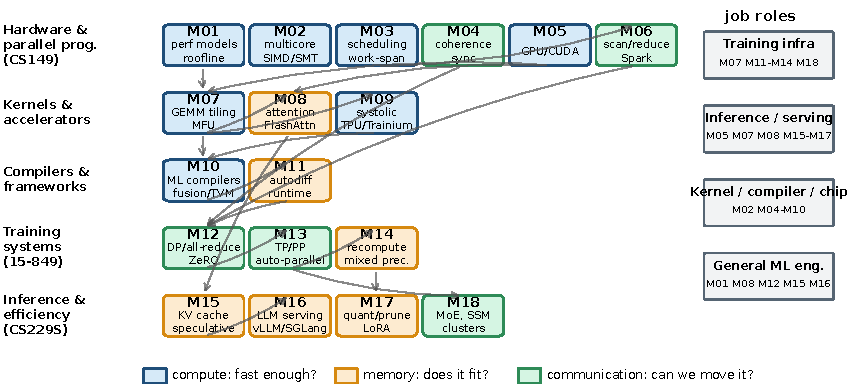
\includegraphics[width=\textwidth]{fig_capability_map}
\caption{18 个模块的知识地图。纵向按系统栈自下而上排列（硬件与并行编程 → 算子与加速器 → 编译器与框架 →
训练系统 → 推理与效率），颜色表示该模块主要回答的问题：蓝色「算得过来」、橙色「放得下」、绿色「传得过来」。
箭头是先修依赖，右侧是四类岗位的主线模块。面试准备时应沿箭头自下而上补齐，而不是按课程顺序线性阅读。}
\label{fig:map}
\end{figure*}

\subsection{三门课程如何互补}

三门课各管一层（表~\ref{tab:modules}）。CS149~\cite{cs149} 讲机器怎么并行：多核、SIMD、GPU、cache coherence、
内存一致性与专用硬件，给「算得过来」打地基。CS229S~\cite{cs229s} 把这些原理用在 Transformer 上：
hardware-aware 算法设计、FlashAttention、KV cache、推测解码、量化与新架构。CMU 15-849~\cite{cmu15849} 是论文研讨课，
覆盖框架、编译器、数据/模型/流水线并行、ZeRO、重计算与压缩，主要回答「放得下」和「传得过来」。
本文不按课程分章，而按系统栈自下而上排成 18 个模块，并补充了课程之后出现、但 2025 年以后推理岗默认要掌握的系统，
例如 vLLM~\cite{kwon2023vllm}、SGLang~\cite{zheng2024sglang}、FlashAttention-3~\cite{shah2024flashattention3}、
chunked prefill~\cite{agrawal2024sarathi} 与 PD 分离~\cite{zhong2024distserve,patel2024splitwise}。

\begin{table*}[!t]
\centering
\caption{18 个模块与三门课程、三个问题和配套实验的对应关系}
\label{tab:modules}
\footnotesize
\begin{tabularx}{\textwidth}{@{}c L{3.6cm} Y Y Y c L{2.6cm}@{}}
\toprule
\# & 模块 & CS149 Fall 2024 & CS229S Fall 2023 & CMU 15-849 S22 & 问题 & 本文配套实验 \\
\midrule
01 & 性能模型与 roofline & Why Parallelism & Hardware-aware algorithm design & Intro to DL systems & 算 & — \\
02 & 多核、SIMD 与多线程 & Multi-core, ISPC & — & — & 算 & CS149 A1 \\
03 & 并行编程与调度 & Work distribution, scheduling & — & — & 算 & CS149 A2 \\
04 & 局部性、一致性与同步 & Coherence, consistency, locks & — & — & 传 & CS149 A2 \\
05 & GPU 架构与 CUDA & GPU architecture, CUDA & GPU 存储层次 & — & 算 & CS149 A3 \\
06 & 数据并行原语 & Data-parallel thinking, Spark & — & Parameter server & 传 & CS149 A3 \\
07 & 矩阵乘与分块 & Efficiently evaluating DNNs & Hardware-aware design & ML hardware & 算 & CS149 A4 \\
08 & Attention 与 FlashAttention & DNN 融合 & FlashAttention & Transformers & 放 & CS229S P1 \\
09 & 专用加速器 & Hardware specialization & — & TPU & 算 & CS149 A4 \\
10 & ML 编译器 & Domain-specific prog. systems & TVM（客座） & ML compilation, TASO & 算 & 15-849 编译 \\
11 & 框架与自动微分 & — & FLOPs 与反传 & Systems for DL & 放 & 15-849 编译 \\
12 & 数据并行与 ZeRO & — & Parallelism fundamentals & Data parallel, ZeRO & 传 & 15-849 分布式 \\
13 & 张量/流水线并行 & — & Narayanan（客座） & Pipeline, Megatron, GSPMD & 传 & 15-849 分布式 \\
14 & 显存优化 & — & Dettmers（客座） & Rematerialization, Offload & 放 & 15-849 分布式 \\
15 & KV cache 与推测解码 & — & Analyzing Transformers & — & 放 & CS229S P2 \\
16 & LLM 推理服务 & — & Scheduling ML clusters & 推理库（客座） & 放 & 15-849 服务 \\
17 & 压缩、量化与 PEFT & — & Memory-efficient NN & Model compression & 放 & 15-849 编译 \\
18 & MoE、SSM、集群与数据 & — & Attention-free, MoE & GNN, ML for systems & 传 & — \\
\bottomrule
\end{tabularx}
\end{table*}

\subsection{本文的定位与贡献}

现有综述大多以「技术谱系」为线索，例如分布式训练综述或推理优化综述。本文的读者是准备 ML infra 面试、
或希望从工程走向研究的工程师，因此组织原则不同：每一个技术点都以「能否当场估算」和「能否说出常见错答」为验收标准。
具体贡献如下：
\begin{enumerate}
\item \textbf{统一的三问题框架}。把 18 个模块的内容组织到式~\eqref{eq:three} 的三项里，使读者能把陌生问题归约到熟悉的估算。
\item \textbf{可复算的数字}。正文中的每个数字要么在文中推导，要么由配套计算器 \texttt{tools/mlsys\_calc.py} 计算
（图表由 \texttt{reports/survey/make\_figures.py} 直接调用该计算器生成），要么引自论文或配套实验 CSV。
\item \textbf{配套实验与诚实的口径}。我们复用了仓库中 9 个 CPU 实验（FlashAttention IO 模型、KV cache 与推测解码、
分布式训练模拟、PagedAttention 服务模拟、编译/自动微分/压缩等）的结果，并逐条标明哪些是正确性验证、哪些是模型输出、
哪些是 CPU 实测，不能外推到 GPU。
\item \textbf{面试能力框架}。第~\ref{sec:interview} 节给出区分工程能力与研究能力的能力矩阵、答题模板、
常见错答清单、把实验转成 STAR 故事的方法以及研究能力练习。
\end{enumerate}

\begin{qa}{面试官为什么总让你「估一下」，而不是直接问概念？}
\ans 概念可以背，估算不行。估算同时检验三件事：是否知道硬件数量级（H100 约 1~PFLOP/s、3.35~TB/s），
是否会把系统行为化成公式（例如 decode 一步至少要读一遍权重），以及是否能从数字推出设计结论（例如 batch 不大时
量化比换卡更有效）。一个合格的回答在 30 秒内给出量级，再说明假设与误差来源。
\wrong 直接报一个经验数字（「大概 100~ms 吧」）而不给推导；或者花 5 分钟推导而不先报结论。
\end{qa}

\subsection{论文组织}

第~\ref{sec:perf} 节建立性能模型；第~\ref{sec:hw} 节讨论并行硬件与 GPU 编程模型；第~\ref{sec:kernel} 节讨论 GEMM、
FlashAttention 与融合；第~\ref{sec:accel} 节讨论专用加速器；第~\ref{sec:compiler} 节讨论编译器与框架；
第~\ref{sec:train} 节讨论分布式训练；第~\ref{sec:infer} 节讨论 LLM 推理与服务；第~\ref{sec:eff} 节讨论模型效率与架构；
第~\ref{sec:cluster} 节讨论集群、可靠性与数据；第~\ref{sec:interview} 节给出面试能力框架；
第~\ref{sec:open} 节讨论开放问题；附录给出公式速查、硬件参数与两周学习计划。
每节末尾有「面试要点」与「研究视角」两个框，前者用于考前复习，后者用于把知识变成可做的实验。
